\subsection{Session 4, Exercise 6}
\label{4_6}

\lineparagraph{Exercise}

Construct a pushdown automaton for the language of palindromes.

\lineparagraph{Solution}

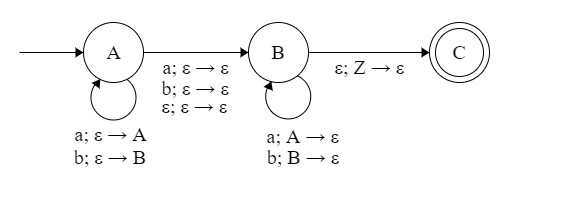
\includegraphics[width=0.5\linewidth]{04/4_6.png}

Proof:

States meaning:
\begin{itemize}
    \item State $A$ is used to read the first half of the word, and store it on the stack.
    \item State $B$ is used to read the second half of the word and compae it to the first half of the word on the stack.
    \item State $C$ can only be reached by emptying the stack out, so only palindromes can reach it.
\end{itemize}

Transitions:

\begin{itemize}
    \item State $A$'s loop transitions will store the corresponding characters on the stack.
    \item Transition from $A$ to $B$ takes care of the middle character, in case of an odd length palindrome, or is an epsilon transition in case of an even length palindrome.
    \item State $B$'s loop transitions will compare the second half of the word with the first half (mirrored, since a stack is a LIFO), and will only remove characters from the input and the stack if they match. If there is a character on the stack that doesn't match the PDA will halt in state $B$, which will reject.
    \item If the stack is emptied out we move to state $C$. In this case, if we read the entire input we can be sure that the word's first half matches the second half, and we will accept. If there are charaters remaining on the input, it means that not the entire word, only the prefix of the word was a palindrome, in which case the PDA correctly rejects, since there is still input remaining.
\end{itemize}

Accept / reject states:

The only accept state is state $C$ which can only be reached with no input remaining if the first half of the input is the mirror of the second half of the input. If a word is not a palindrome there won't be any accepting branch in the computation, all branches will end up in either $A$ (store the entire word), or $B$: start comparing too late, stack is not empty to move to $C$, or $C$ but with input remaining, since we started comparing too early.